% !TeX spellcheck = en_US
\chapter{Methodology}\label{chap: Meth}%
This chapter describes the methodologies of general \gls{mas} design. 
The general \gls{mas} is distributed into internal (\ref{chap: Meth-Internal}) and external (\ref{chap: Meth-External}) parts,  
with a \gls{mas} for \gls{cda} and \gls{ra} as an internal and \gls{dta} as an external system. 
These two systems are decoupled from each other but still under the concept of agent based operation system. 
At the end, it concludes the timing properties for both 
internal and external systems with protocols in 
different layers and proposes an assumption of modularizing transport 
delay with a visual notation.
\section{Internal}\label{chap: Meth-Internal}
In this section, the design pattern for \gls{mas} is chosen and the tasks of each module within is discussed.
After that, the characteristics of transport layer protocols and application layers protocols are compared. 
Eventually the methodologies of using python WebSocket for \gls{mas} and RESTful API for one to one agent communication are listed in pseudocode. 

\subsection{Overview (conceptual diagram)}

%figure conceptual MAS
\begin{figure}[htb]
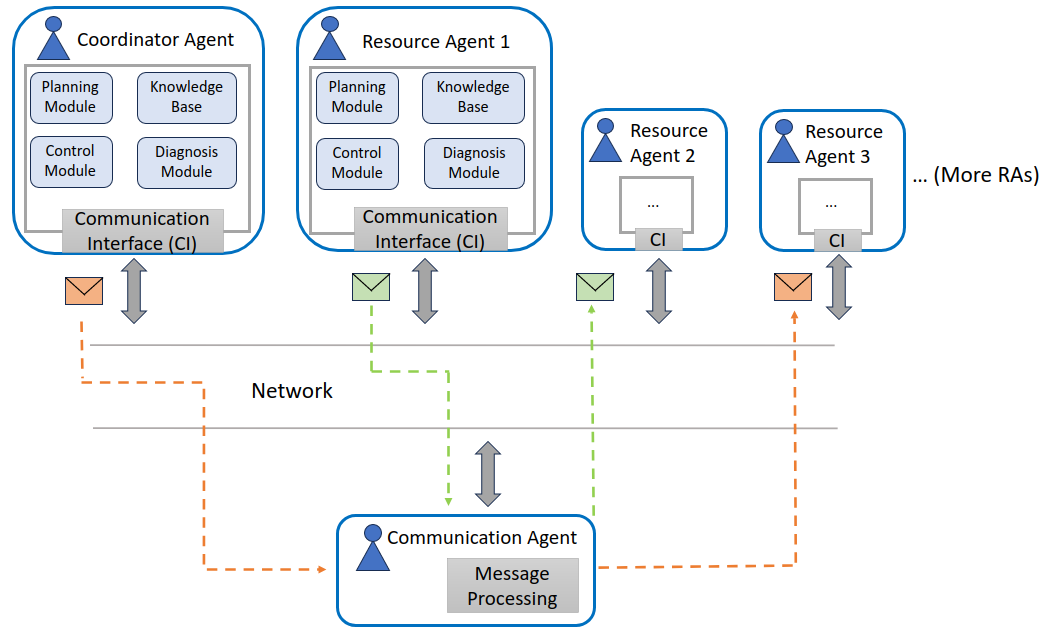
\includegraphics[width=\textwidth]{figures/MAS_Conceptual_Diagram.png}
\centering
\caption{Conceptual diagram of MAS\label{fig: MASConceptual}}
\end{figure}

% decribe the conceptual diagram

The fig.\ref{fig: MASConceptual} shows a conceptual diagram of a \gls{mas} based on the \gls{ra} design patterns in Wannagat’s architecture, with the focus on communication between agents, planning and decision making inside each agent. The \gls{cda} here is identical to \gls{ams} of Wanagat, which should also be counted as an agent instead of a management system. The five modules within an agent are: 
\begin{itemize}
    \item Planning Module
    \item Control Module
    \item Knowledge Base
    \item Diagnosis Module
    \item Communication Interface
\end{itemize}

for both \gls{cda} or a \gls{ra}.
Based on these five modules, the task to be executed in an agent should also be categorized into 5 parts. The following tab.\ref{tab:designPatterns} shows some tasks of each module based on the general requirements of a smart factory.


\begin{table}[p]
    \setlist[itemize]{leftmargin=*, topsep=0pt, itemsep=2pt, parsep=0pt}
    \caption{Wanagat's \gls{ra} design patterns with task related examples.}
    \label{tab:designPatterns}
    \small
    \renewcommand{\arraystretch}{1.2} 
    \setlength{\extrarowheight}{3pt}
    \centering
    \begin{tabularx}{\textwidth}{|Y|Z|W|}
    \hline
    \multicolumn{3}{|c|}{Wanagat's design patterns} \\ 
    \hline
    Module name & Task & Example \\ 
    \hline
    Planning Module &
    \vspace{-10pt}    
    \begin{itemize}
        \item Task planning 
        \item Decision making 
        \item Resource allocation 
        \item Sequencing 
        \item Scheduling
    \end{itemize} 
    &  
    \vspace{-10pt}   
    \begin{itemize}
        \item Break down tasks into smaller executable units
        \item Decide which task should be assigned to which agent 
        \item Allocate the agents with specific tasks 
        \item Find the task execution sequence 
        \item Calculate the execution time for each agent
    \end{itemize} \\
    \hline
    
    Control Module & 
    \vspace{-10pt}
    \begin{itemize}
        \item Monitoring 
        \item Adaptation 
        \item Control and optimization 
        \item Resource allocation 
        \item Actuation
    \end{itemize}
    & 
    \vspace{-10pt}
    \begin{itemize}
        \item Acquisition of robot states
        \item Adapt the plans with current state (e.g., emergent stop) 
        \item Control and optimize the robot's motion 
        \item Allocate the agents with specific tasks 
        \item Actuate the robot with outputs
    \end{itemize} \\
    \hline
    
    Knowledge Base & 
    \vspace{-10pt}
    \begin{itemize}
        \item \gls{db}
        \item Knowledge representation and reasoning 
        \item Learning 
        \item Knowledge sharing 
    \end{itemize}
    & 
    \vspace{-10pt}
    \begin{itemize}
        \item Hierarchical, relational, non-relational and object oriented
        \item Relational ontology \gls{db} system
        \item Agent learns from the existing primitives and create new executable primitives for customer's changing requirements
        \item Unfound primitives could be retrieved by querying other agents
    \end{itemize} \\
    \hline

    Diagnosis Module & 
    \vspace{-10pt}
    \begin{itemize}
        \item Fault detection 
        \item Fault diagnosis 
        \item Fault prediction 
        \item Root cause analysis and classification
    \end{itemize}
    & 
    \vspace{-10pt}
    \begin{itemize}
        \item Hierarchical, relational, non-relational and object oriented
        \item Relational ontology \gls{db} system
        \item Agent learns from the existing primitives and create new executable primitives for customer's changing requirements
        \item Unfound primitives could be retrieved by querying other agents
    \end{itemize} \\
    \hline

    Communication Interface & 
    \vspace{-15pt}
    \begin{itemize}
        \item Message parsing and encoding
        \item Connection establishment, maintenance
        \item Message handling 
        \item Data security
    \end{itemize}
    & 
    \vspace{-15pt}
    \begin{itemize}
        \item Encode and decode the massages in agent specific data type, or  parse the data object to other types (e.g., json)
        \item Ensure the connection with other agents based on system requirements
        \item Filter messages with undesired data type or incomplete messages, prioritize the incoming messages
        \item Ensure data integrity and confidentiality by encrypting, decrypting and authenticating messages
    \end{itemize} \\
    \hline
    \end{tabularx}
    \end{table}


\subsection{Prerequisite}
\subsubsection{System Setup}
 
%figure conceptual MAS
\begin{figure}[htbp]
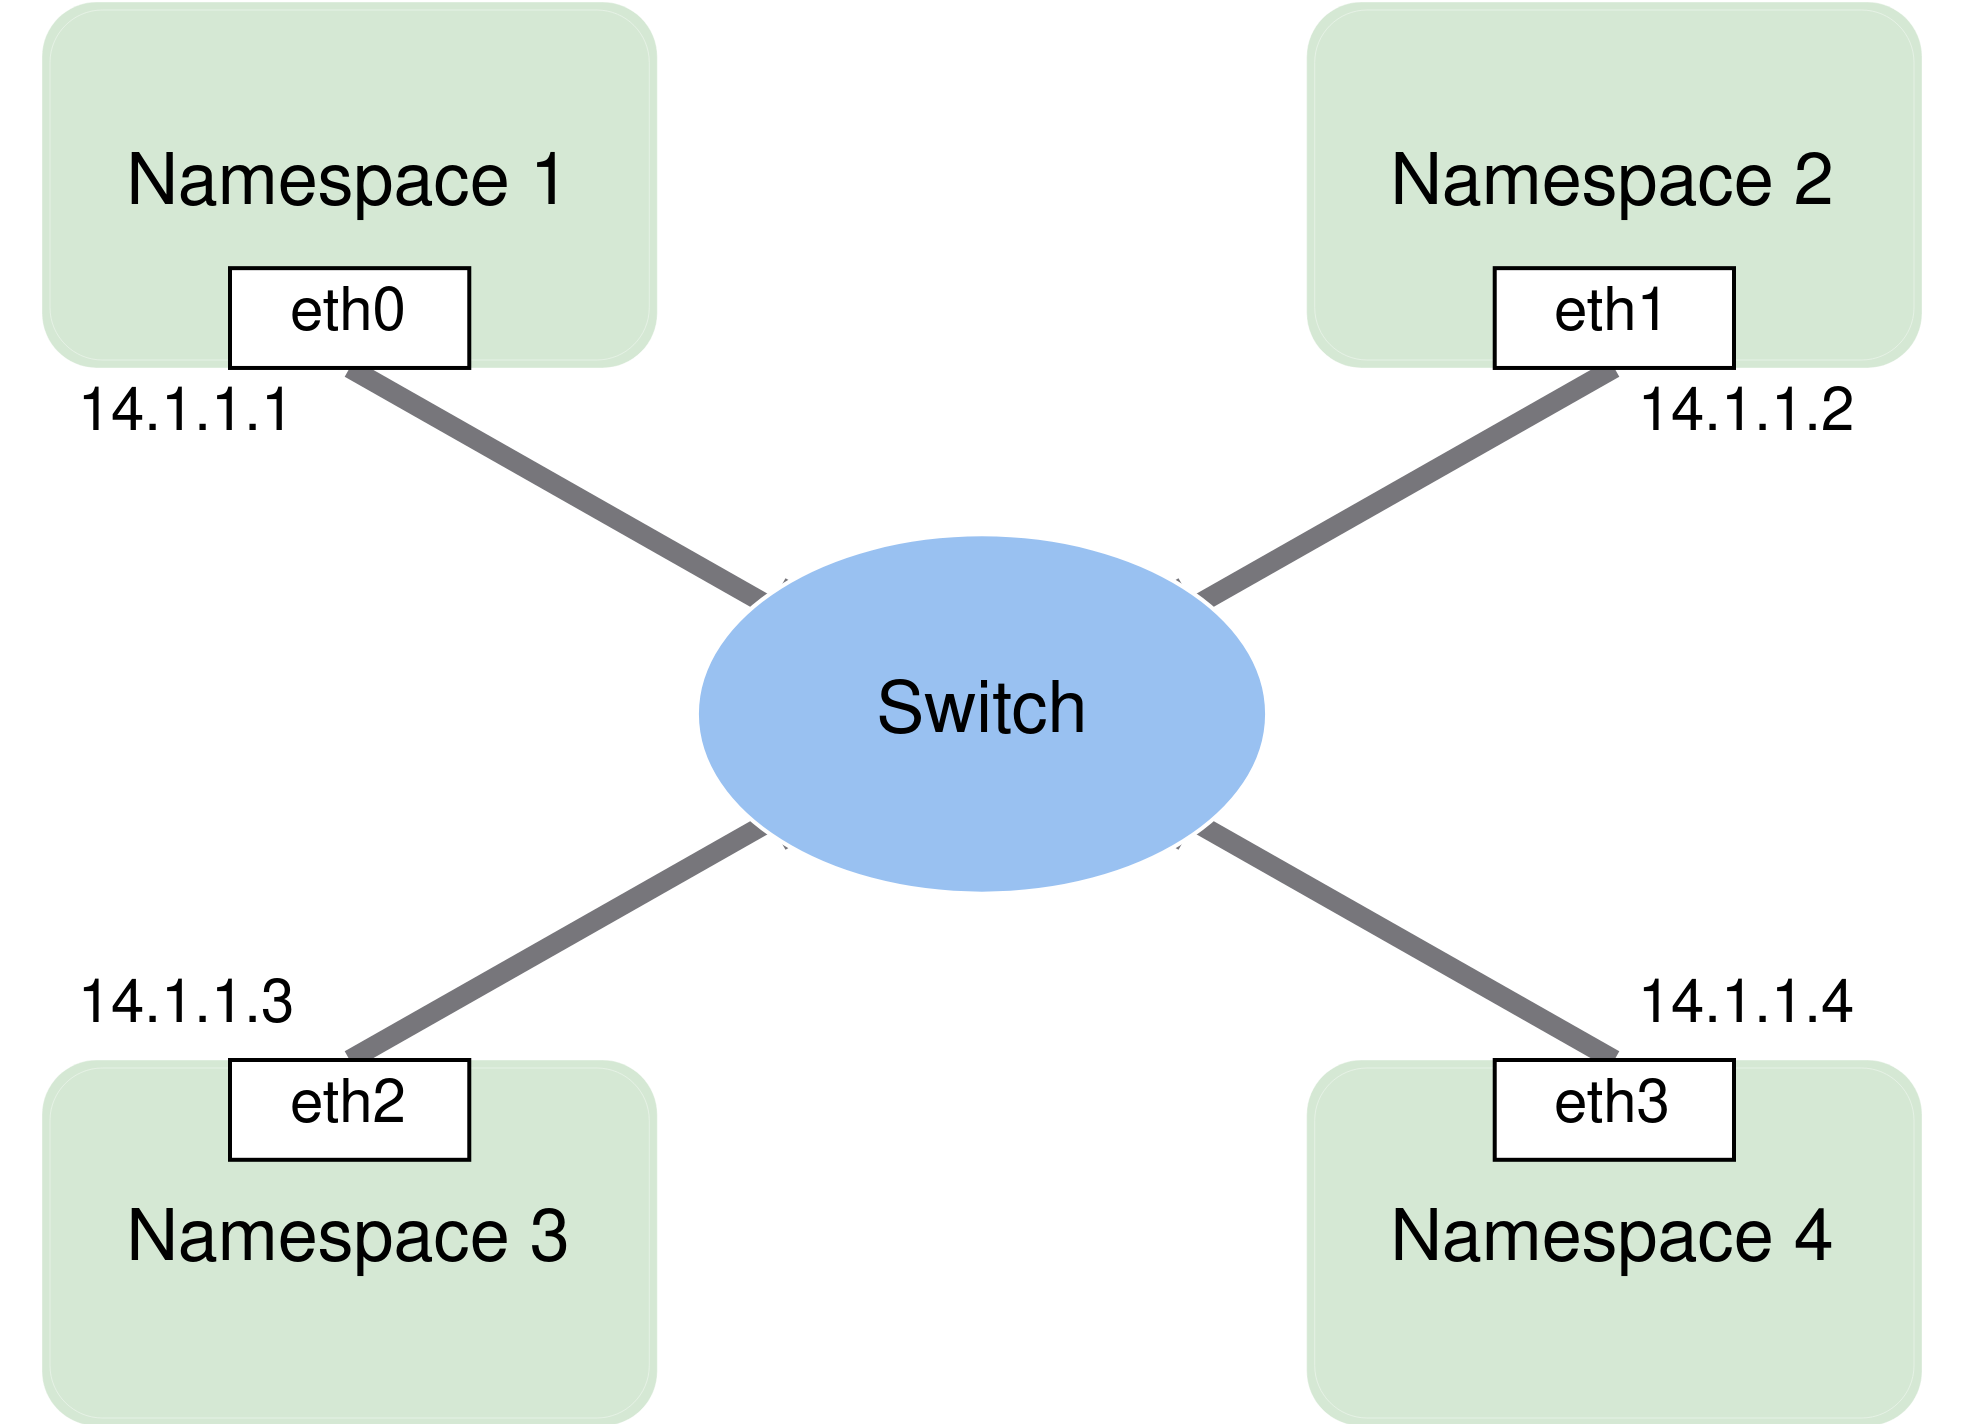
\includegraphics[width=0.8\textwidth]{figures/NamespaceConceptual.png}
\centering
\caption{Conceptual diagram of namespaces creation
\label{fig: NSConceptual}}
\end{figure}

In order to emulate network environments for agent's communication testing 
and development of the \gls{mas}, the internal packets routing between 
agents in a single Linux device should be avoided. A common way to 
visualize the network to do performance testing is to use namespaces 
for network emulation. The trick is that a process running within a given 
namespace will see only the network interfaces, including virtual 
interfaces, forwarding tables, etc., that exist in that namespace. 
The applications under test should serve as a switch and each packet 
should be routed through these interfaces. The fig.\ref{fig: NSConceptual} 
shows that, each namespace is assigned with a virtual ethernet interface, 
starting with the name eth, which is configured with an individual IP 
address. Each time a script gets called, it is running under a namespace 
with its own IP address. In exercise, if a packet is sent from Namespace 1 
to Namespace 3 and then back, it is routed by the switch intead of bridges 
between namespaces, which are not configured here in order to avoid 
internal routing.

\subsection{\gls{osi} model and comparison between sockets relevant protocol layers}
%figure conceptual MAS
\begin{figure}[htbp]
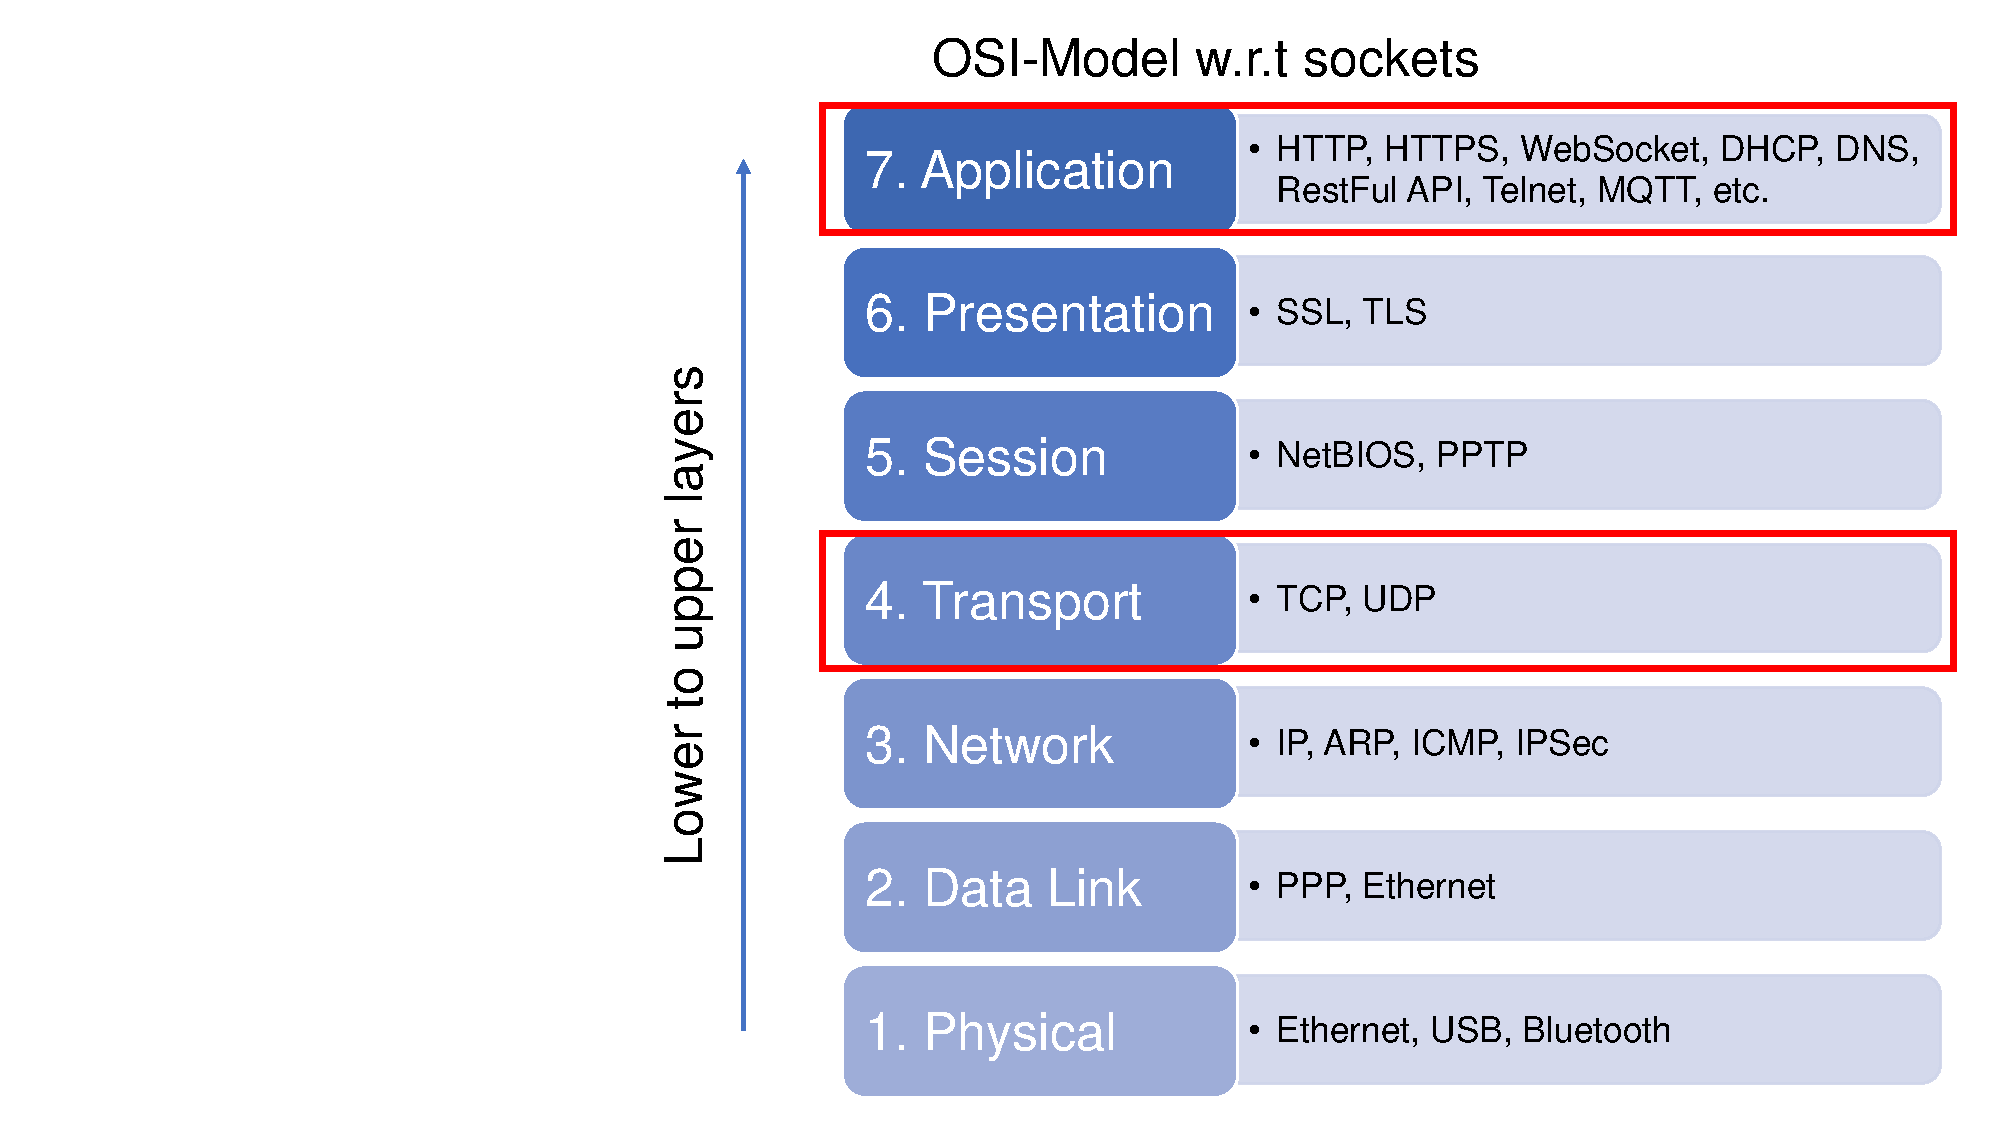
\includegraphics[width=0.8\textwidth]{figures/OSI.pdf}
\centering
\caption{\gls{osi} model with example protocols \label{fig: OSI}}
\end{figure}

Fig.\ref{fig: OSI} shows the famous \gls{osi} model with 7 abstraction layers with Transport layer and application layers most relevant to sockets. 
TCP and UDP are typical transport layer protocols and they provide an end-to-end data transport between two devices while the application layer protocols like HTTP or Websocket establish a communication between applications within devices. 
Although the application layer protocols still utilize TCP/UDP sockets to transport stream data, they defined additional "rules" to specify structure, content, and semantics of the messages transport through sockets. 
In the following tables, a comparison between protocols in different layers provide a more straight forward overview of their pro and cons in different contents.


\subsubsection{Transport layer protocols}
Tab.\ref{tab: transportlayer} compares the typical transport layer protocols \gls{tcp} and \gls{udp} from different aspects.  
\gls{tcp} provides reliable data transfer while \gls{udp} mainly focuses on transport speed and efficiency without reliability guarantee. 
With the focus on speed and reliability, \gls{udp} on one hand offers a faster packet transfer, while on the other hand produces a network dependent packet loss rate and out-of-order packet sequence, compared to \gls{tcp}. 
Because of the requirement of a reliable real time ordered data transfer with minimum to no packet loss in \gls{mas} communication, TCP is used as the base protocols of the design. 


\begin{table}[htbp]
    \small
    \centering
    \caption{Characteristics of different technologies in transport layer protocols}
    \label{tab: transportlayer}
    \begin{tabular}{|m{0.2\textwidth}|m{0.3\textwidth}|m{0.3\textwidth}|}
    \hline
    \multicolumn{3}{|c|}{\textbf{Transport layer protocols}}                                                            \\ \hline
    \textbf{Aspect}                         & \textbf{\gls{tcp}}             & \textbf{\gls{udp}}        \\ \hline
    Use cases                      & Web browsing, email, text messaging, and file transfers & Live and real-time data transmission \\ \hline
    Reliability                    & Reliable        & Unreliable \\ \hline
    Stream type                    & Byte stream with no preserved boundaries & Message stream with preserved boundaries \\ \hline
    Connection type                & Connection oriented, three handshake & No connection needed \\ \hline
    Overhead                       & Larger than \gls{udp} & Very low   \\ \hline
    Sequence                       & Packets arrive in sequence & No sequencing for packets \\ \hline
    Retransmission of lost packets & Yes             & No         \\ \hline
    Speed                          & Slower than \gls{udp}, because of overhead and connection & Relative faster than \gls{tcp} \\ \hline
    State                          & Stateful        & Stateless  \\ \hline
    Flow control                   & Yes             & No         \\ \hline
    \end{tabular}
    \end{table}




\subsubsection{Application layer protocols}


% % Please add the following required packages to your document preamble:

\begin{sidewaystable}[p]
    \small
    \caption{Characteristics of different technologies in application layer protocols}
    \label{tab: applicationlayer}
    \centering
    \begin{tabular}{|m{0.13\textwidth}|m{0.2\textwidth}|m{0.2\textwidth}|m{0.2\textwidth}|m{0.2\textwidth}|}
    \hline
    \multicolumn{5}{|c|}{\textbf{Application layer protocols}} \\ \hline
    \textbf{Aspect} & \textbf{HTTP} & \textbf{WebSocket} & \textbf{RESTful API} & \textbf{MQTT} \\ \hline
    Use cases & Web pages, images, videos, World Wide Web, etc & Such as chat applications, live gaming, etc & Web and mobile applications with data management requirement & Usually in IoT with limited bandwidth \\ \hline
    Functionality & Request-response protocol based on TCP, foundation for both RESTful APIs and the initial connection in WebSockets & Bi-directional, real-time communication & Uses standard HTTP methods to perform CRUD (Create, Read, Update, Delete) & Lightweight message transport, runs over TCP \\ \hline
    Security & Use SSL/TLS & ws (unsecured) and wss (secured with SSL/TLS) & Similar to HTTP, can be further secured using various authentication mechanisms like OAuth, JWT & Use TLS, like username/password authentication and optional message-level security \\ \hline
    Message patterns & Request-Response & Full Duplex (send and receive independent) & Request-Response & Publish-Subscribe \\ \hline
    Connection type & No connection needed & Persistent {connection} & No connection needed & Persistent connection \\ \hline
    State & Stateless & Stateful & Stateless & Stateful \\ \hline
    Overhead & Overhead for each request-response cycle, especially for new connections & After the initial handshake (HTTP), data frames are lightweight & Similar to HTTP, dependent on API design & Minimal message overhead \\ \hline
    Realtime capability & Less Capable & Highly Suitable & Variable & Highly Suitable \\ \hline
    Flexibility & Supported in all environments & Supported in most modern web browsers and many backend environments & Similar to HTTP & Highly flexible \\ \hline
    Adaptability to dynamic changes & Relative lower (influenced by stateless nature) & High & Relative lower (influenced by stateless nature) & High \\ \hline
    Capability of handling instability & Less capable, requires a stable connection for each request-response cycle & Less stable if connection disruptions happen frequently & Identical to HTTP & Capable, Ideal for remote locations with limited connectivity \\ \hline
    Scalability & Less scalable, require more infrastructure support & Highly scalable, maintains connections for real-time interactions & similar to HTTP, dependent on API design & Highly scalable based on broker-client message transport \\ \hline
    \end{tabular}
\end{sidewaystable}

There are several protocols in application layers that are considered to be suitable for \gls{mas} communication, each with its own advantages and limits in different aspects according to tab.\ref{tab: applicationlayer}.
To get a closer look of the tab.\ref{tab: applicationlayer}, a horizontal comparisons between different application layer protocols: 

\begin{itemize}
    \item \gls{http}
    \item WebSocket
    \item RESTful API
    \item and \gls{mqtt}
\end{itemize}

should be performed. In one word, WebSocket is chosen to be the application layer protocols for MAS communication, while \gls{tcp} socket for the \gls{dta} design, which will be further discussed in the next chapter. Here are the reasons of the choice of WebSocket: 

\begin{itemize}
    \item Bi-directional, full duplex, real time communication between server and clients, no re-connection needed, suitable for continuous data transfer
    \item Small overhead after connection establishment to reduce latency (\gls{http})
    \item Stateful, store the information of the client's state under connection
    \item High flexibility, adaptability and scalability
    \item Secure with wss
\end{itemize}

Fig.\ref{fig: MsgConceptual} shows the differences between bi-directional full duplex and other message patterns like Request-Response and Publish-Subscribe, in the context of data transfer. 
For the \gls{mqtt}, publisher publish (send) a message within a topic to the broker (server), while subscriber subscribes (receive) the message from the broker within the same topic. 
For response, a new topic needed to be started, but there is no guarantee that the original publisher is listening, which is a drawback for send-and-receive patterns of \gls{mas}. 

Relatively, the other three protocols will be considered as more appropriate. 
For instance both HTTP and RESTful API run in request-response mechanism. 
A client posts (sends) messages to the server for the other client will get (receive) from it. 
Whether the GET and POST method are successful or not, a response will be given back. With this mechanism, each time a message is going through the server, a new connection will be established and closed after responses are sent. 
The inconsistent connection will consume more communication time and lead to higher latency. 
The ideal solution for that is the bi-directional and full duplex real time communication mechanism of WebSocket. 
Basically the client sends a message to the server, after processing the data, the server will pass the message to the other client and receive response with the same logic. This allows simultaneous communication in both directions between clients, so that no re-connection in the message transfer cycle is necessary. The consistent server-client connection makes it possible to realize a continuous real time communication between agents. In the next section, a more detailed explanation of WebSocket mechanism for \gls{mas} design will be given.

%figure conceptual application layer protocols
\begin{figure}[htb]
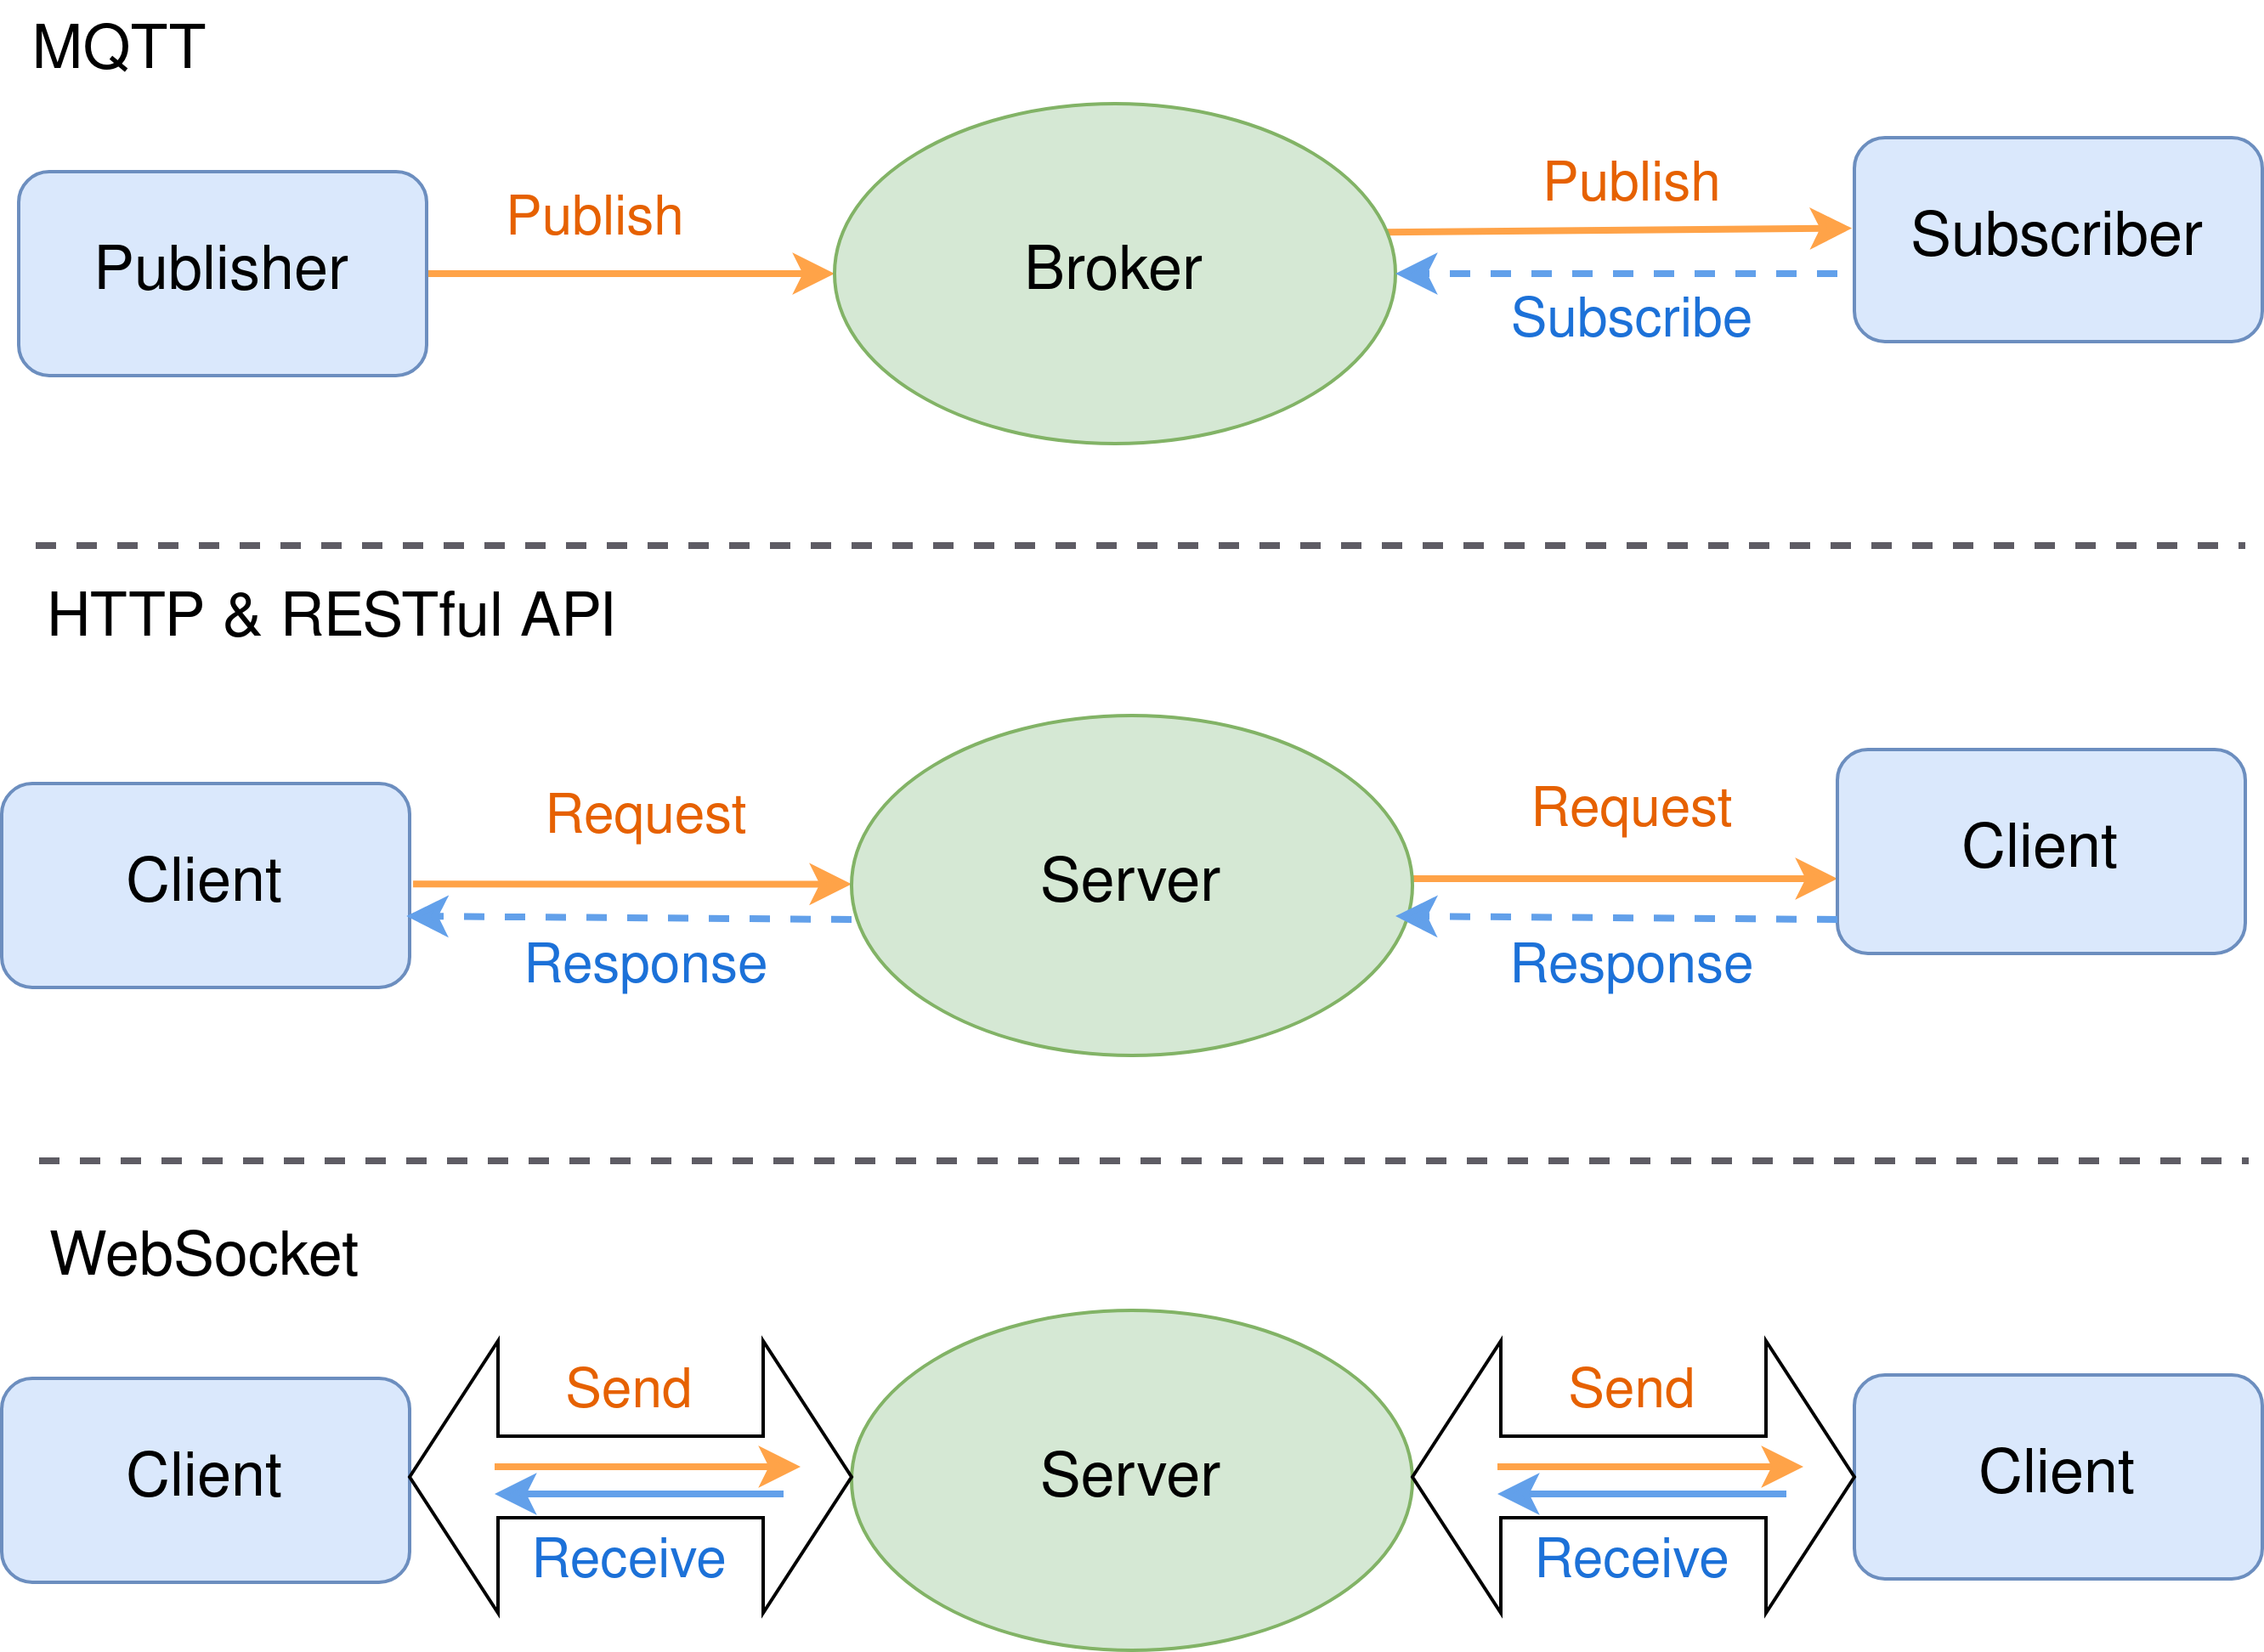
\includegraphics[width=0.8\textwidth]{figures/MessageConceptual.png}
\centering
\caption{Conceptual diagram of different applcation layer 
protocols\label{fig: MsgConceptual}}
\end{figure}

\subsection{Transport layer protocols versus Application layer protocols}
The reasons of choosing application layer protocols over transport layer protocols for \gls{mas} according to table \ref{tab: transportlayer} and \ref{tab: applicationlayer} are listed as following:
\begin{itemize}
    \item Semantic-rich message patterns
    \item Higher flexibility
    \item Standardized communication between different agents
    \item Header with agent relevant information
    \item Security and authentication
    \end{itemize}
However, unlike for \gls{mas} design, the architecture of \gls{dta} is more straightforward and the basic \gls{tcp} socket is chosen for the more to one server-client communication. 
The details will be discussed later in section \ref{chap: Meth-External}.

\subsection{Pseudo-Code of MAS workflow in WebSocket python}
In algorithm \ref{alg: CDAPseudoCode} is a piece of pseudocode that reflects the workflow of the \gls{mas} for the \gls{cda}. 
Unlike other \gls{ras}, \gls{cda} has no mechanisms of primitives execution but the ability to do planning and decision making. 
Under the Main, the production tasks are broken down into a set of sequenced primitives and then assigened to each allocated agent through one of the predefinded $send\_and\_receive()$ functions under the messageSender class.
After getting responses from the agents, \gls{cda} should deicide whether to start processing by positive responses or retry the steps by negative responses.  
Once the process starts, the \gls{cda} does nothing but wait for the inform messages from the allocated agents by using one of the $receive\_and\_send()$ functions under the messageReceiver class. 
This allows \gls{cda} to have an overall control among the entire prodution process with the purpose of centralization of the distributed agent systems.  


As for the decentralization of \gls{mas}, the \gls{ra} should be able to react to \gls{cda} and do decision making for its own field level control.  
Which means, \gls{cda} should only be informed about the status of the production process, while the exact processes should be done within \gls{ra} and the material flow should be informed between \gls{ras}. The combination of centralization and decentralization will save the resource power consumed by \gls{cda}, 
while still maintains the management level control and decision making.  
The algorithm \ref{alg: RAPseudoCode} shows the logic of a \gls{ra}. At the beginning, \gls{ra} waits for the connection and capability check from \gls{cda}, after that first agent in the list of $sequenced\_agent$ will listen to the starting message from \gls{cda}, 
and other agents, will wait for the availability check and inform message of the last agent in the list. 
After executing all primitives of its own, the \gls{ra} should check the availability and inform the starting point of next agent.  
Once all primitives in the list are done, the last agent should inform the \gls{cda} about the end of processing.


Before the agents start to run, the WebSocket server program (algorithm \ref{alg: ServerPseudoCode}) must be started first, so that the messages from agents will be routed to it, which serves as a \gls{ca}.  
The server runs asychronously and listen to incoming messages forever. 
Which means, every time a new agent gets connected to the server, a new thread will be started and killed after the incoming message is processed and sent to the recipient agent. 
All threads run concurrently and the maximal possible connection number is limited by the hardware and also the network bandwidth and latency. 
After the server receives a message, it should first identify the message type to check whether it is in json or string format. 
After that, it will either split the string or parse the json file to retrieve the recipient name, the priority and the message content. 
Since all message handling processes run concurrently, there is a chance that multiple messages coming in the server and waiting for processing at the same time. 
In order to rearrange them and handle the messages with higher priority first, all messages should be pushed to queue and the critical messages should be popped out first, after this the important and then normal messages. 
Finally the message will be either processed further or sent directly to the recipient. 

   
\begin{breakablealgorithm}
\caption{Pseudo-Code for \gls{cda} in MAS workflow}
\label{alg: CDAPseudoCode}
\begin{algorithmic}[1]
\State \textbf{Input:} custRequirement
\State {Import} WebSocket
\State {Initialize} agentID, centralServerIP
\State \textbf{Class} messageSender
    \State \textbf{\qquad function} {$send\_and\_receive(self, recipient, message, priority)$}
    \State \qquad \qquad Establish a WebSocket connection    
    \State \textbf{\qquad \qquad while} recipient not Found \textbf{do}    
    \State \qquad \qquad \qquad Send prioritized messages and wait for response

    \State \textbf{\qquad function} {$send\_capCheck\_and\_receive(self, recipient, primitive, priority)$}
    \State \qquad \qquad Establish a WebSocket connection
    \State \textbf{\qquad \qquad while} recipient not found \textbf{do} 
    \State \qquad \qquad \qquad Send prioritized messages and wait for response
    \State \qquad \qquad \qquad Handle capability exceptions

    \State \textbf{\qquad function} {$send\_image\_and\_receive(self, recipient, image\_path, priority)$}
    \State \qquad \qquad {\#similar to $send\_and\_receive()$ but send an image }    
    % \State \qquad \qquad ...

    \State \textbf{\qquad function} {$send\_availCheck\_and\_receive(self, recipient, primitive, priority)$}
    \State \qquad \qquad {\#similar to $send\_capCheck\_and\_receive()$ but raise availibility exceptions } 
    % \State \qquad \qquad ...

\State \textbf{EndClass}
\State \textbf{Class} messageReceiver
    \State \textbf{\qquad function} {$receive\_and\_send(self, response, priority)$}
    \State \qquad \qquad Establish a WebSocket connection
    \State \textbf{\qquad \qquad while} message not received \textbf{do}
    \State \qquad \qquad \qquad Receive, process and send responses with priority
    \State \textbf{\qquad function} {$receive\_image\_and\_send(self, response, priority)$}
    \State \qquad \qquad {\#similar to $receive\_and\_send()$ but receive and save an image }    
    % \State \qquad \qquad ...    
    \State \textbf{EndClass}
\State \textbf{Class} agentsAllocation
    \State \textbf{\qquad function} {$allocate\_agents\_with\_seq\_primitives(self, requirements)$}
    \State \qquad \qquad Find tasks from customer requirements
    \State \qquad \qquad Breakdown tasks into skills into primitives
    \State \qquad \qquad Create sequence lists for primitives and agents allocation    
    \State \qquad \qquad \textbf{return} sequences
    \State \textbf{EndClass}
\State \textbf{Main:}
\State {\qquad Instantiate} agentsAllocation, messageSender and messageReceiver with agentID
\State \qquad $sequences = allocate\_agents\_with\_seq\_primitives(custRequirement)$
\State \qquad \textbf{repeat}
\State \qquad \qquad $send\_and\_receive(agent, connectMsg, priority)$
\State \qquad \textbf{until} all allocated agents connected
\State \qquad \textbf{repeat}
\State \qquad \qquad $send\_capCheck\_and\_receive(agent, primitive, priority)$
\State \qquad \textbf{until} all allocated agents capable of all primitives
\State \qquad \textbf{repeat}
\State \qquad \qquad $send\_and\_receive(agent, sequences, priority)$
\State \qquad \textbf{until} all allocated agents receive sequences
\State \qquad \qquad $send\_availCheck\_and\_receive(1st\_Agent, 1st\_primitive, priority)$
\State \qquad \textbf{repeat}
\State \qquad \qquad $receive\_and\_send(responseMsg, priority)$
\State \qquad \textbf{until} informed by last agent with finish message 
\State \textbf{End} 
\end{algorithmic}
\end{breakablealgorithm}

%pseudo code for RA
\begin{breakablealgorithm}
    \caption{Pseudo-Code for \gls{ra} in MAS workflow}
    \label{alg: RAPseudoCode}
    \begin{algorithmic}[1]
    \State {Import} WebSocket
    \State {Initialize} agentID, centralServerIP, subServerIP
    
\State \textbf{Class} messageSender
    \State \textbf{\qquad function} {$send\_and\_receive(self, recipient, message, priority)$}
    \State \qquad \qquad Establish a WebSocket connection    
    \State \textbf{\qquad \qquad while} recipient not Found \textbf{do}    
    \State \qquad \qquad \qquad Send prioritized messages and wait for response

    \State \textbf{\qquad function} {$send\_availCheck\_and\_receive(self, recipient, primitive, priority)$}
    \State \qquad \qquad Establish a WebSocket connection
    \State \textbf{\qquad \qquad while} recipient not found \textbf{do} 
    \State \qquad \qquad \qquad Send prioritized messages and wait for response
    \State \qquad \qquad \qquad Handle availability exceptions

    \State \textbf{\qquad function} {$send\_image\_and\_receive(self, recipient, image\_path, priority)$}
    \State \qquad \qquad{\#similar to $send\_and\_receive()$ but send an image }
    % \State \qquad \qquad ...

\State \textbf{EndClass}

\State \textbf{Class} messageReceiver
    \State \textbf{\qquad function} {$receive\_and\_send(self, response, serverID)$}
    \State \qquad \qquad Establish a WebSocket connection
    \State \textbf{\qquad \qquad while} message not received \textbf{do}
    \State \qquad \qquad \qquad Receive, process and send responses with priority
    \State \textbf{\qquad function} {$receive\_capCheck\_and\_send(self, response, serverID)$}
    \State \qquad \qquad Establish a WebSocket connection
    \State \textbf{\qquad \qquad while} message not received \textbf{do}
    \State \qquad \qquad \qquad Receive, check capability and send responses with priority
    \State \qquad \qquad \qquad Handle capability exceptions
    \State \textbf{\qquad function} {$receive\_sequences\_and\_send(self, response, serverID)$}
    \State \qquad \qquad Establish a WebSocket connection
    \State \textbf{\qquad \qquad while} message not received \textbf{do}
    \State \qquad \qquad \qquad Receive, store sequences and send responses with priority

    \State \textbf{\qquad function} {$receive\_image\_and\_send(self, response, serverID)$}
    \State \qquad \qquad{\#similar to $receive\_and\_send()$ but receive and save an image }    
    % \State \qquad \qquad ...    
    \State \textbf{\qquad function} {$receive\_availCheck\_and\_send(self, response, serverID)$}
    \State \qquad \qquad {\#similar to $receive\_capCheck\_and\_send()$ but check availability}
    % \State \qquad \qquad ...  
    \State \textbf{EndClass}
 

   
    \State \textbf{Main:}
    \State {\qquad Instantiate} messageSender and messageReceiver with agentID
    \State \qquad $receive\_and\_send(connectMsg, centralServerID)$
    \State \textbf{\qquad repeat}
    \State \qquad \qquad $receive\_capCheck\_and\_send(capMsg, centralServerID)$
    \State \textbf{\qquad until} CapabilityCheck finished  
    \State \textbf{\qquad for} agent in sequence {\textbf do}
    \State \textbf{\qquad \qquad if} {agent is first in sequence} \textbf{then}
        \State {\qquad \qquad \qquad} $receive\_availCheck\_and\_send(availMsg, centralServerID)$
        \State \textbf{\qquad \qquad else}
        \State \textbf{\qquad \qquad \qquad if} {previous agent is not self} \textbf{then}
            \State \qquad \qquad \qquad \qquad $receive\_availCheck\_and\_send(availMsg, SubServerID)$
            \State \qquad \qquad \qquad \qquad executePrimitive(primitive)
        
            \State \textbf{\qquad \qquad \qquad if} {agent is not last one AND next agent is not self} \textbf{then}
            \State \textbf{\qquad \qquad \qquad \qquad} $send\_availCheck\_and\_receive(nextAgent, primitive, priority)$
            \State \textbf{\qquad \qquad \qquad \qquad} executePrimitive(primitive)
            \State \textbf{\qquad \qquad \qquad \qquad} $send\_and\_receive(nextAgent, informMsg, priority)$
         
            \State \textbf{\qquad \qquad \qquad if} {agent is last} \textbf{then}
            \State \textbf{\qquad \qquad \qquad \qquad} executePrimitive(primitive)
            \State \textbf{\qquad \qquad \qquad \qquad} $send\_and\_receive(\gls{cda}, informFinishMsg, priority)$
            \State \textbf{\qquad end for} 
    \State \textbf{End} 
\end{algorithmic}
\end{breakablealgorithm}


%pseudo code for Server
\begin{breakablealgorithm}
    \caption{Pseudo-Code for \gls{ca} as a server in MAS workflow}
    \label{alg: ServerPseudoCode}
    \begin{algorithmic}[1]
        \State {Import} WebSocket
        \State {Initialize} serverID, priorityDict, messageQueue, connectedAgents
        \State \textbf{Do in parallel}
        \State \textbf{\qquad function} handler(WebSocket, path)  
        \State \textbf \qquad \qquad receive agent name and store in connectedAgents
        \State \textbf {\qquad \qquad while} WebSocket connected \textbf{do} 
        \State \textbf \qquad \qquad \qquad receive message from agent   
        \State \textbf{\qquad \qquad \qquad if} {message is json} \textbf{then}
        \State \textbf \qquad \qquad \qquad \qquad parse json message and retrieve recipient
        \State \textbf \qquad \qquad \qquad \qquad store agent messages in messageQueue  
        \State \textbf \qquad \qquad \qquad \qquad $process\_jsonMessage(recipient, jsonMsg)$
        \State \textbf{\qquad \qquad \qquad else}  
        \State \textbf \qquad \qquad \qquad \qquad retrieve recipient from string message
        \State \textbf \qquad \qquad \qquad \qquad store agent messages in messageQueue  
        \State \textbf \qquad \qquad \qquad \qquad $process\_message(recipient, stringMsg)$
        
        \State \textbf{\qquad function} $process\_message(recipient, stringMsg)$   
        \State \textbf \qquad \qquad prioritize messages from priorityDict and store in messageQueue 
        \State \textbf \qquad \qquad handle messages with higher priority first   
        \State \textbf \qquad \qquad send stringMsg to recipient 
        \State \textbf{\qquad function} $process\_jsonMessage(recipient, jsonMsg)$   
        \State \textbf \qquad \qquad prioritize messages from priorityDict and store in messageQueue
        \State \textbf \qquad \qquad handle messages with higher priority first 
        \State \textbf \qquad \qquad send jsonMsg to recipient
        \State \textbf{Main:}   
        \State \textbf {\qquad while} true \textbf {do}
        \State \textbf \qquad \qquad handler(WebSocket, serverID) 
        \State \textbf{End}                 
    \end{algorithmic}
\end{breakablealgorithm}

\subsection{Pseudo-Code of one to one agent communication workflow in RESTful API}
A more comparable application layer protocol is RESTful API, which has the request-response mechanism with more addtional functionalities compared to \gls{http}. 
Therefore RESTful API was considered as an alternative of communication protocol other than WebSocket. 
However, based on some test results in chapter \ref{chap: Result}, WebSocket is 
proved to be more appropriate.
As a result, different from WebSocket, the design of RESTful API based system is only built for performance testing and comparison with WebSocket.
Therefore, the RESTful API system is simplified to be an one to one agent communication without other functionalities like decision making or message prioritization, etc.

According to the pseudo code for agentSR (send and receive messages) and 
agentRS (receive and send messages) in 
algorithm \ref{alg: SRPseudoCode} and \ref{alg: RSPseudoCode}, and the server 
in algorithm \ref{alg: apiServerPseudoCode}, 
the basic mechanism is similar to the one designed for WebSocket. One major 
difference is that, the connection will be closed after the message is sent 
from the clientSR to clientRS.
If the agentRS needs to send a response message back to inform the success, 
re-connection is needed. 
Instead of send and receive from WebSocket, agentSR first POST a request to the server to call the function $send\_message()$, 
while agentRS GET a request to the server for the function call $get\_message()$, same for the reverse direction. 
Under the same condition, the message transfer routine with RESTful API will possibly results in more latency than WebSocket, which will be verified later.
  
\begin{algorithm}
    \caption{Pseudo-Code for agentSR in one to one communication workflow}
    \label{alg: SRPseudoCode}
    \begin{algorithmic}[1]
    \State {Import} flask
    \State {Initialize} agentID, serverIP
        \State \textbf{function} {$send\_and\_receive(sender, recipient, msg)$}
        \State \qquad format msg with agent IDs 
        \State \qquad post request msg to server
        \State \textbf{\qquad while} no response \textbf{do}    
        \State \qquad \qquad {$wait\_for\_response(sender, recipient)$}

        \State \textbf{function} {$wait\_for\_response(sender, recipient)$}
        \State \textbf{\qquad while} message not received \textbf{do}    
        \State \qquad \qquad get request jsonMsg from server and wait for reponse
        \State \qquad \qquad parse jsonMsg to retrieve message content
    

    \State \textbf{Main:}
    \State \qquad {$send\_and\_receive(agentID, recipient, msg)$}
    \State \textbf{End} 
    \end{algorithmic}
    \end{algorithm}


    \begin{algorithm}
        \caption{Pseudo-Code for agentRS in one to one communication workflow}
        \label{alg: RSPseudoCode}
        \begin{algorithmic}[1]
        \State {Import} flask
        \State {Initialize} agentID, serverIP
            \State \textbf{function} {$send\_message(recipient, msg)$}
            \State \qquad format msg with recipient ID 
            \State \qquad post request msg to server and wait for response 
    
            \State \textbf{function} {$get\_message(agentID)$}  
            \State \qquad get request jsonMsg from server and wait for response
            \State \qquad parse jsonMsg to retrieve message content
            \State \qquad \textbf{return} msg, recipient         
    
        \State \textbf{Main:}
        \State \qquad {$msg, recipient = get\_message(agentID)$}
        \State \textbf{\qquad if} msg AND recipient \textbf{then}   
        \State \qquad \qquad{$send\_message(recipient, msg)$}
        \State \textbf{End} 
        \end{algorithmic}
        \end{algorithm}

    \begin{algorithm}
        \caption{Pseudo-Code for a server in one to one communication workflow}
        \label{alg: apiServerPseudoCode}
        \begin{algorithmic}[1]
        \State {Import} flask
        \State {Initialize} jsonMsg 
        \State \textbf{Class} app
            \State \qquad \textbf{function} {$send\_message()$}
            \State \qquad \qquad {\# POST request in app class} 
            \State \qquad \qquad parse the json file from request
            \State \qquad \qquad retrieve recipient and message content 
            \State \qquad \qquad \textbf{if} recipient AND msgContent \textbf{then}
            \State \qquad \qquad \qquad jsonify senderIP and message content and store in jsonMsg
            \State \qquad \qquad \qquad response is OK status code
            \State \qquad \qquad \textbf{else}            
            \State \qquad \qquad \qquad response is Error code            
            \State \qquad \qquad \textbf{return} response  

            \State \qquad \textbf{function} {$get\_message(agentID)$}  
            \State \qquad \qquad {\# GET request in app class} 
            \State \qquad \qquad \textbf{if} agentID in jsonMsg \textbf{then}
            \State \qquad \qquad \qquad send jsonMsg and response is OK status code
            \State \qquad \qquad \textbf{else}
            \State \qquad \qquad \qquad response is Error code
            \State \qquad \qquad \textbf{return} response         
    
        \State \textbf{Main:}
        \State \qquad Instantiate app
        \State \qquad run app forever
        \State \textbf{End} 
        \end{algorithmic}
        \end{algorithm}

\section{External} \label{chap: Meth-External}
As for the external \gls{dta} system, the data flow will be visualized in section \ref{chap: Overview-External}.
After that, the \gls{ntp} setup for delay measurement between local devices and cloud will
be explained in section \ref{chap: ntpsetup}. For a better understanding of the workflow, 
the pseudo code of \gls{rcp} and \gls{dta} is provided in section \ref{chap: RCPDTAPseudo}. 
Finally, the Azure Digital Twin platform set up for data ingestion will be explained
in the last section.



\subsection{Overview (conceptual diagram)}\label{chap: Overview-External}

%figure conceptual DT
\begin{figure}[htb]
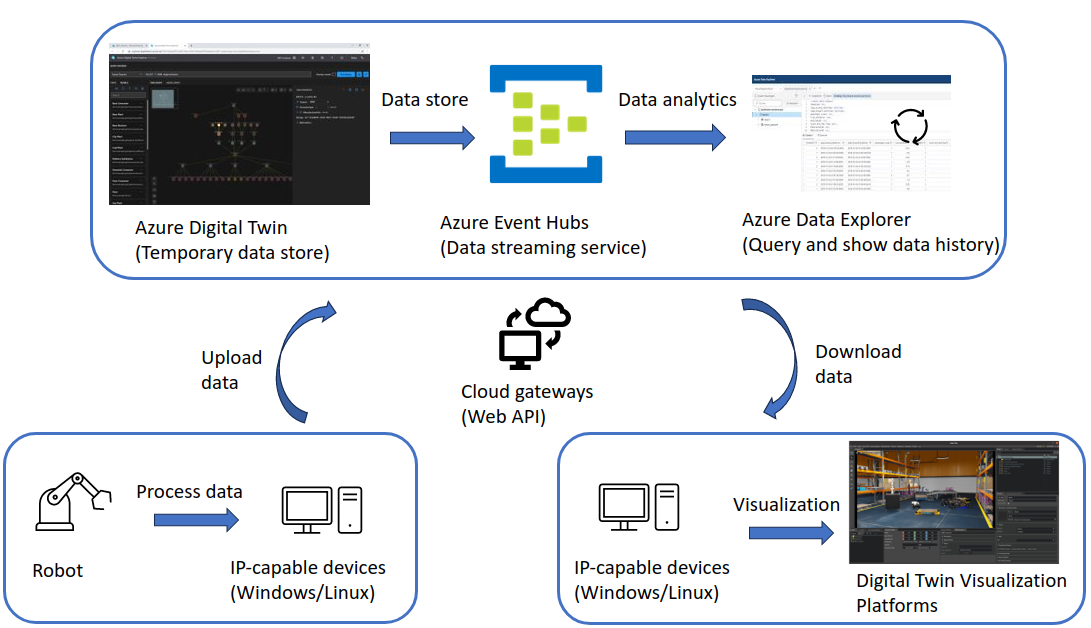
\includegraphics[width=\textwidth]{figures/DT_Conceptual_Diagram.png}

\centering
\caption{Conceptual diagram of MAS\label{fig: DTConceptual}}
\end{figure}

The fig.\ref{fig: DTConceptual} shows the workflow of \gls{dta} updating global digital twin.
The process begins from the left hand side of the graph. The \gls{dta} receives process data constantly from robots, including steady state data. 
After the separating the sticky packets from \gls{tcp} socket, the process data will be parsed and uploaded one by one to the \gls{ms} Azure Digital Twins cloud. 
All the updates of the digital twin instances in cloud will be shown in Azure Digital Twins Explorer temporarily and stored in Azure Event Hubs concurrently. 
After that the history data could be ingested for further analysis in Azure Data Explorer. 
The Azure Digital Twins Explorer here serves as a monitor of robot status while the Azure Data Explorer as a data analysis tool. 
Once the remote data update is successful, the data will be downloaded to local host immediately and may be further used as inputs of any other visualization purposes. 
Within this upload and download cycle of data, the real time capability should also be maintained.  


It is worth mentioning that, the process data is produced by robot motion which makes the \gls{dta} completely decoupled from the \gls{mas}. 
The advantages of the decoupling is that, even though there is a complete disorder of the \gls{mas}, the current robot states will be recorded and updated in remote, 
which is beneficial for data acquisition and monitoring. 



\subsection{Prerequisite} \label{chap: ntpsetup}
\subsubsection{\gls{ntp} setup}
In order to measure the delays between local host and cloud, the clock of both end must be synchronized. 
Due to the nature of computer systems, the software clock might drift away from the "true" time (absolute \gls{utc} time) due to various reasons like system load, hardware imperfections, or even temperature changes.
Therefore, before the measurement, the software clock of local host should be synchronized with the global clock using \gls{ntp}. 
The NTP setup of linux system are:  

\begin{enumerate}
    \item System update and upgrade.
    \item Install \gls{ntp}.
    \item Add reliable global \gls{ntp} servers/server pools to configure ntp.conf file.
    \item Allow port 123/udp for or disable firewall.
    \item Restart \gls{ntp} and check \gls{ntp} status.
    \item Check synchronization status (e.g.: reach, delay, offset and jitter, etc).
    \end{enumerate}

Since the cloud system clock is already synchronized with \gls{utc} time, all the tests and calculations results are based on UTC time. 

\subsection{Pseudo-Code of \gls{rcp} and \gls{dta} workflow in C++ and C\#}\label{chap: RCPDTAPseudo}

As mentioned at the beginning of this chapter, \gls{dta} should be completely decoupled from \gls{mas}. 
In the following algorithm \ref{alg:RCPPseudoCode} and \ref{alg:DTAgentPseudoCode}, the workflows of \gls{rcp} and \gls{dta} are listed separately.
In the \gls{rcp} workflow, the robot arm is controled by a set of predefined functions with a possibility to record the current states. 
Each time when a new state is recorded, it should be sent to the \gls{dta} immediately through the established \gls{tcp} socket.
As for the \gls{dta} side, it should be started before \gls{rcp}, and listen to the socket to receive data stream once connected.
Each time when a new connection to a \gls{ra} is created, the \gls{dta} will create a new thread, to receive, process, upload and download data concurrently.
One issue of using \gls{tcp} is that, packets do not arrive one by one but stuck to each other, which is solved by using delimiter for packets separation.  



%pseudo code for RCP
\begin{breakablealgorithm}
    \caption{Pseudo-Code of \gls{rcp} workflow}
    \label{alg:RCPPseudoCode}
    \begin{algorithmic}
    \State {Import} socket, franka
    \State {Initialize} \gls{dta}\_IP
    \State \textbf{function} {$get\_rstate\_and\_send(clientSocket)$}
        \State \qquad Start robot motion and record robot state
        \State \qquad {$send\_message(robotState, clientSocket)$}
    \State \textbf{function} {$send\_message(msg, clientSocket)$}
        \State \qquad send robot state to \gls{dta} 
    \State \textbf{Main:}
    \State \qquad Instantiate robot
    \State \qquad Initialize start position
    \State \qquad Establish a \gls{tcp} connection with \gls{dta}  
    \State \qquad {$get\_rstate\_and\_send(clientSocket)$}
    \State \textbf{End}
    \end{algorithmic}
\end{breakablealgorithm}


%pseudo code for DTAgent
\begin{breakablealgorithm}
    \caption{Pseudo-Code of \gls{dta} workflow}
    \label{alg:DTAgentPseudoCode}
    \begin{algorithmic}
    \State {Import} socket, AzureDigitalTwin
    \State {Initialize} \gls{rcp}\_IP(s)
    \State \textbf{function} {$read\_and\_upload\_download\_processData(\gls{rcp}\_IP)$}
        \State \qquad \textbf{do run in parallel}
            \State \qquad \qquad $create\_client\_thread(\gls{rcp}\_IP)$       
    \State \textbf{function} {$create\_client\_thread(\gls{rcp}\_IP)$}
        \State \qquad Establish a \gls{tcp} connection with \gls{ra}
        \State \qquad {$data = read\_data(clientSocket)$}  
        \State \qquad {$process\_data\_upload\_and\_download(data)$}    
    \State \textbf{function} {$read\_data(clientSocket)$}
        \State \qquad receive and store robot state data
        \State \qquad \textbf{return} data
    \State \textbf{function} {$process\_data\_upload\_and\_download(data)$}
        \State \qquad separate sticky packets with delimiter
        \State \qquad upload processed data to Azure Digital Twins in json patch
        \State \qquad download twin after data update 
    \State \textbf{Main:}
        \State \qquad \textbf{for} \gls{rcp}\_IP in IPs \textbf{do}
        \State \qquad \qquad {$read\_and\_upload\_download\_processData(\gls{rcp}\_IP)$}
        \State \textbf{End}
    \end{algorithmic}
\end{breakablealgorithm}



\subsection{Azure Digital Twins}
According to the workflow described in section \ref{chap: Overview-External}, 
a stable and functional Azure Digital Twins platform should be set up to ensure
the data flow, including Azure Digital Twins Explorer, Azure Event Hub and Azure
Data Explorer. Azure Digital Twins instance is configured with a time series data 
history connection. Other resources must also be created such as an Event Hubs 
namespace, an event hub, Azure Data Explorer cluster, and a database. 
After a connection, data is sent to an event hub which eventually forwards 
the data to the Azure Data Explorer cluster and stored in a database.The history 
data includes twin property updates, twin lifecycle events and relationship lifecycle 
events, which can be later queried in Azure Data Explorer.
\subsubsection{Setup}
Here is the sequence of the basic setup in the Azure platform:
\begin{enumerate}
    \item Create Azure Event Hub namespace and add instance.
    \item Create Azure Data Explorer cluster and add database.
    \item Connect data history of the Event Hub instance to the digital twin instance.
\end{enumerate}

In order to verify whether the connection is successful, one can try updating the 
digital twin instance and querying data from the Azure Data Explorer side. The query
language is called \gls{kql}, which is powerful for patterns discovery, anomalies 
and outliers identification, and statistical modeling (various graphs creation). 
Following algorithm \ref{alg: KQLCode} is a snippet of the example \gls{kql} code in the test: 

\begin{algorithm}
    \caption{\gls{kql}}
    \label{alg: KQLCode}
    \begin{algorithmic}
        \State  AdtPropertyEvents 
        \State {| where ID == 'RadPositionJoint3' and Key == 'value'}
        \State {| where TimeStamp between (datetime(2023-08-27 16:02) .. datetime(2023-08-27 19:00))}
        \State {| order by TimeStamp asc}
        \State {| project TimeStamp, Id, Key, Value}
    \end{algorithmic}
\end{algorithm}


\begin{figure}[htb]
    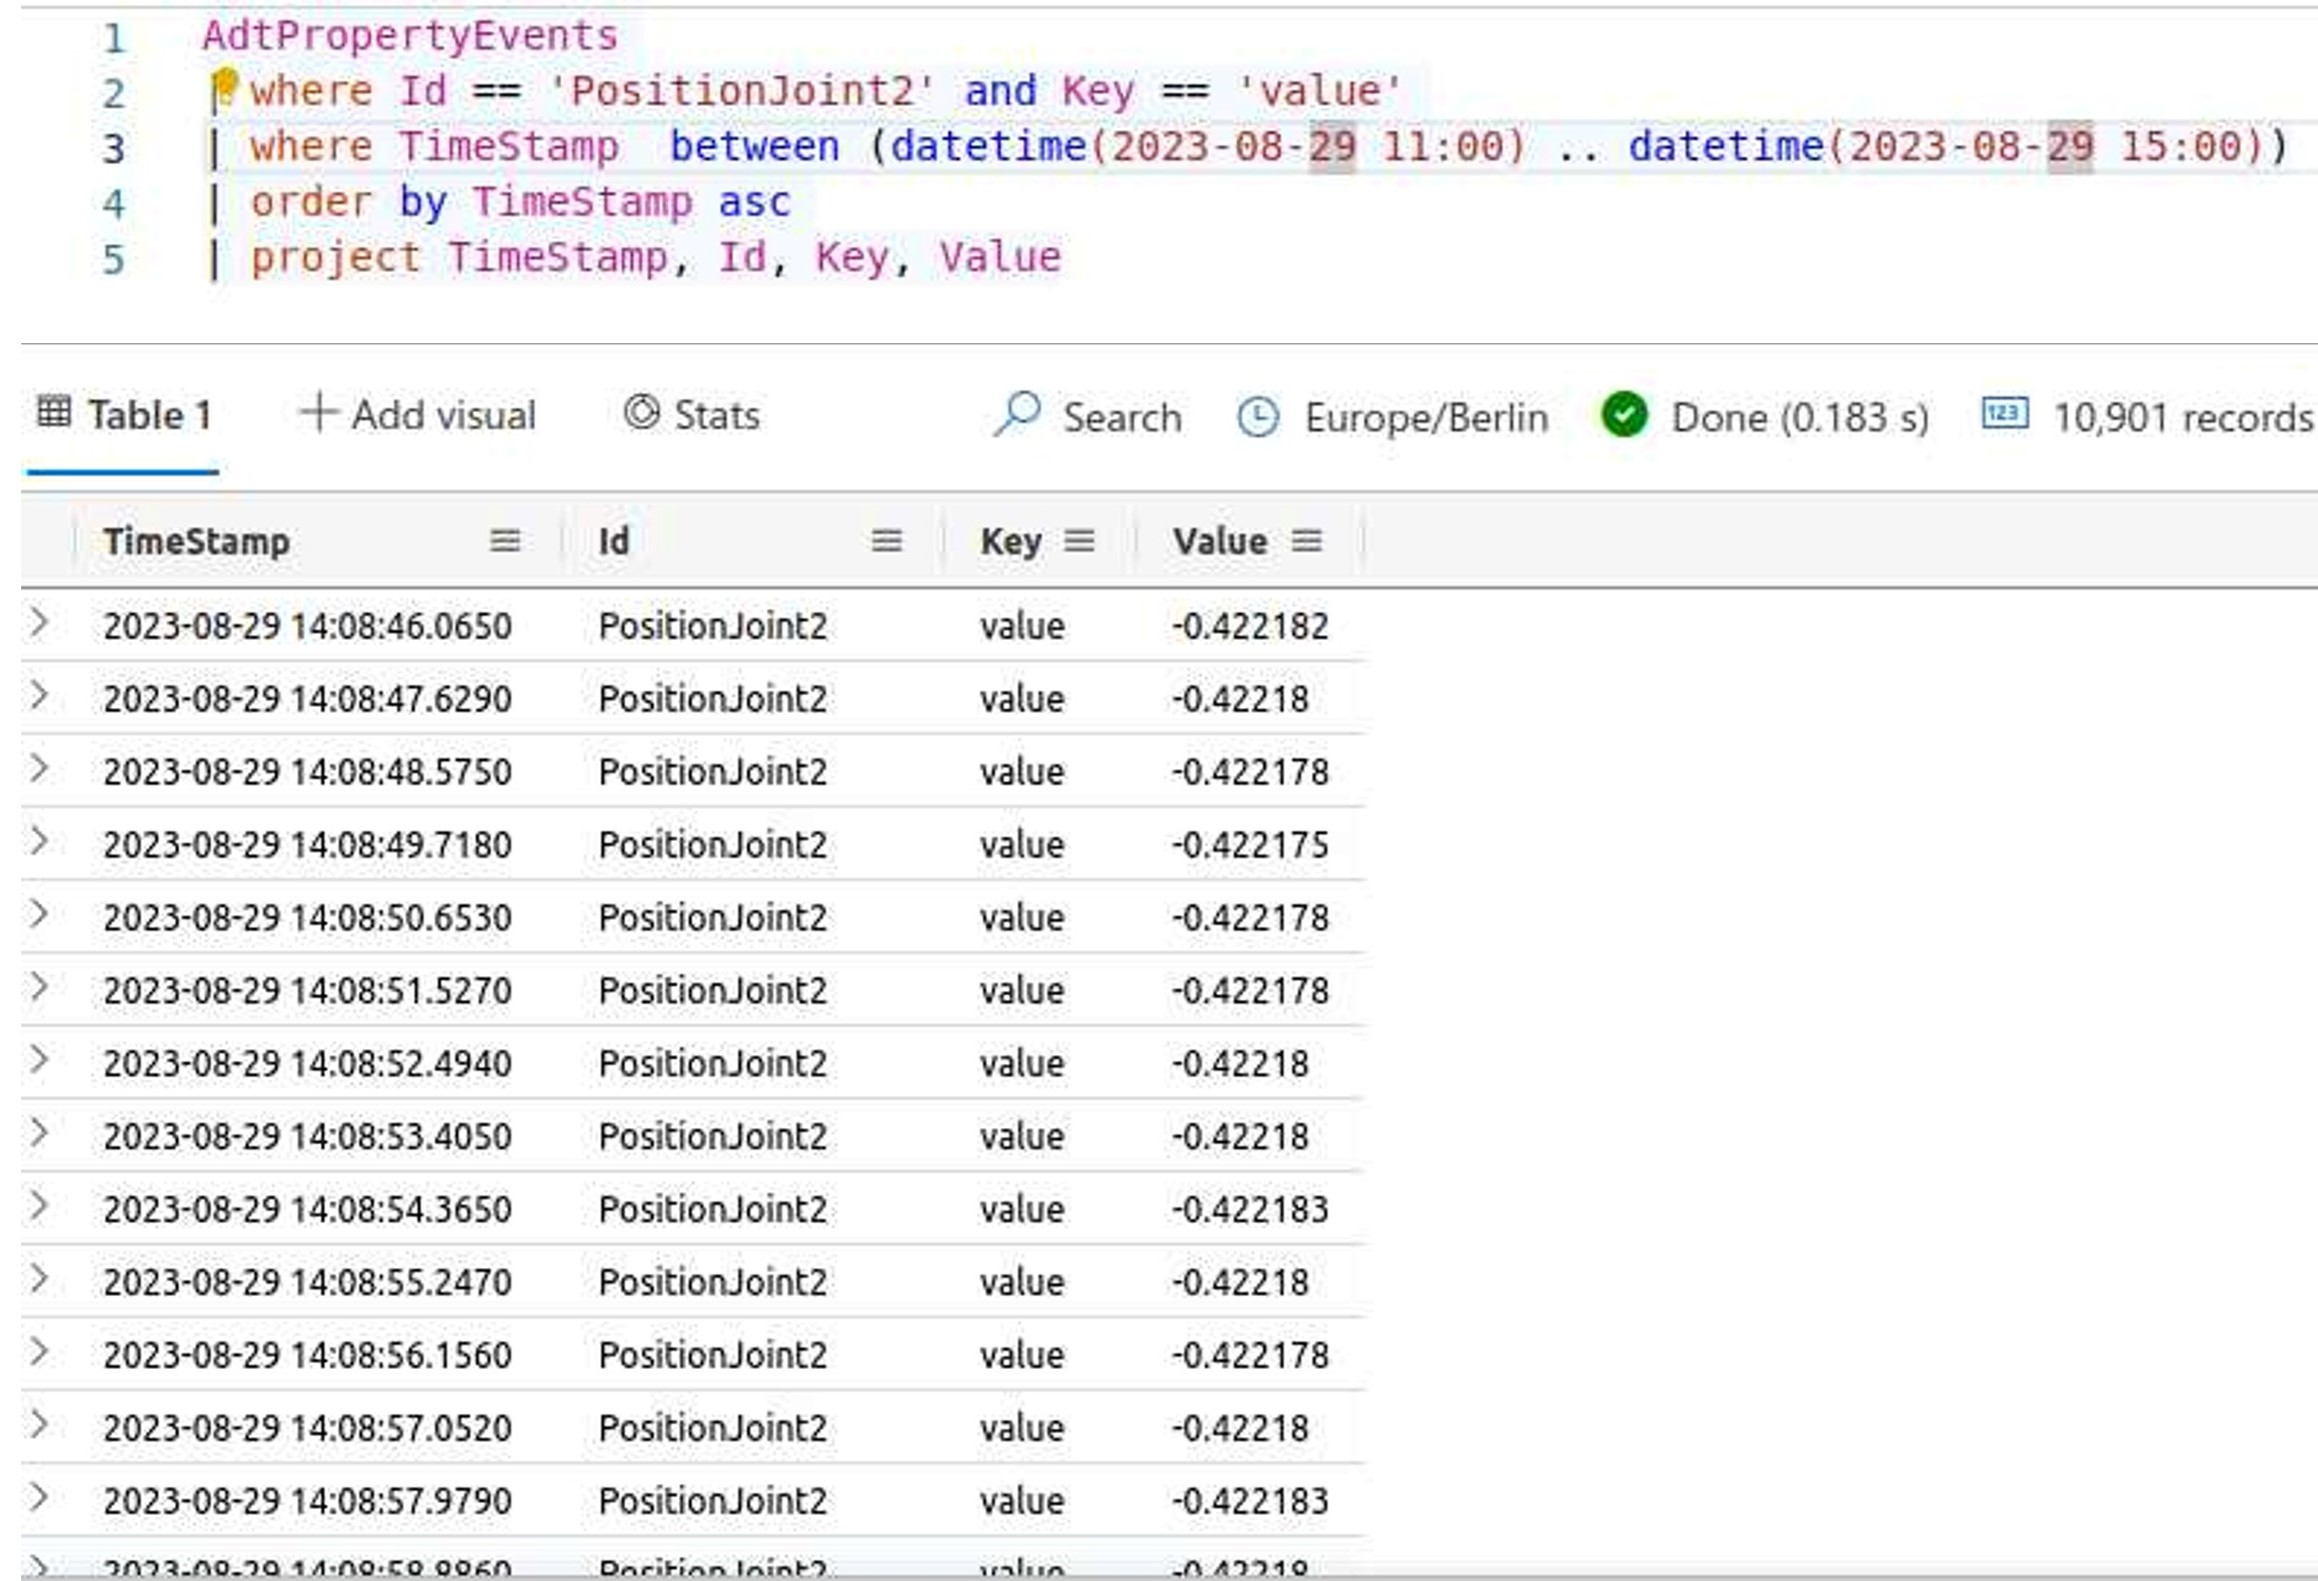
\includegraphics[width=\textwidth]{figures/KQL_cut.jpg}
    
    \centering
    \caption{Snippet of Data Explorer\label{fig: KQL}}
\end{figure}

As shown in fig.\ref{fig: KQL}, by executing the code from the snippet, all the history data will be listed as a table 
which can be downloaded to local later. 


\section{Modularization}\label{chap: Meth-Modular}
In addition to the internal and external designs of a general \gls{mas}, 
there are also some considerations of modularizing timing behaviors of the 
system. In the following sections, the \gls{tcp/ip} model as well as 
\gls{dsl} will be introduced and used as design basis of a modularized general 
\gls{mas}. 
\subsection{From \gls{osi} model to \gls{tcp/ip} model}

Despite the fact that \gls{tcp} being categorized as a transport layer protocol 
according to the fig.\ref{fig: OSI}, the data transfer
between different \gls{tcp} sockets should also go through all layers. 
The reason is that, the \gls{tcp} socket will be operated by a program 
using socket libraries, which is an operation under application layer. 
The transport layer protocols does nothing but accepting data from session layer 
in \gls{osi} model, and truncate it into smaller pieces to ensure a reliable and correct
data transport. However, it will be too strict and complecated 
to consider delays in all seven 
layers for modularization purposes. Therefore, the concentration should be 
shifted from the general \gls{osi} model to the more abstract \gls{tcp/ip} model 
as depicted in fig.\ref{fig: TCP_IP}. 


The \gls{tcp/ip} model consists of four layers: application layer, tansport layer, 
internet layer and network access layer, with each mapping different layers in 
\gls{osi} model. As depicted in \gls{tcp/ip} model, 
the application layer roughly contains the upper three layers while the network access layer 
contains the physical and data link layer. The network layer is renamed as internet layer, 
while transport layer remains the same. 

\begin{figure}[htb]
    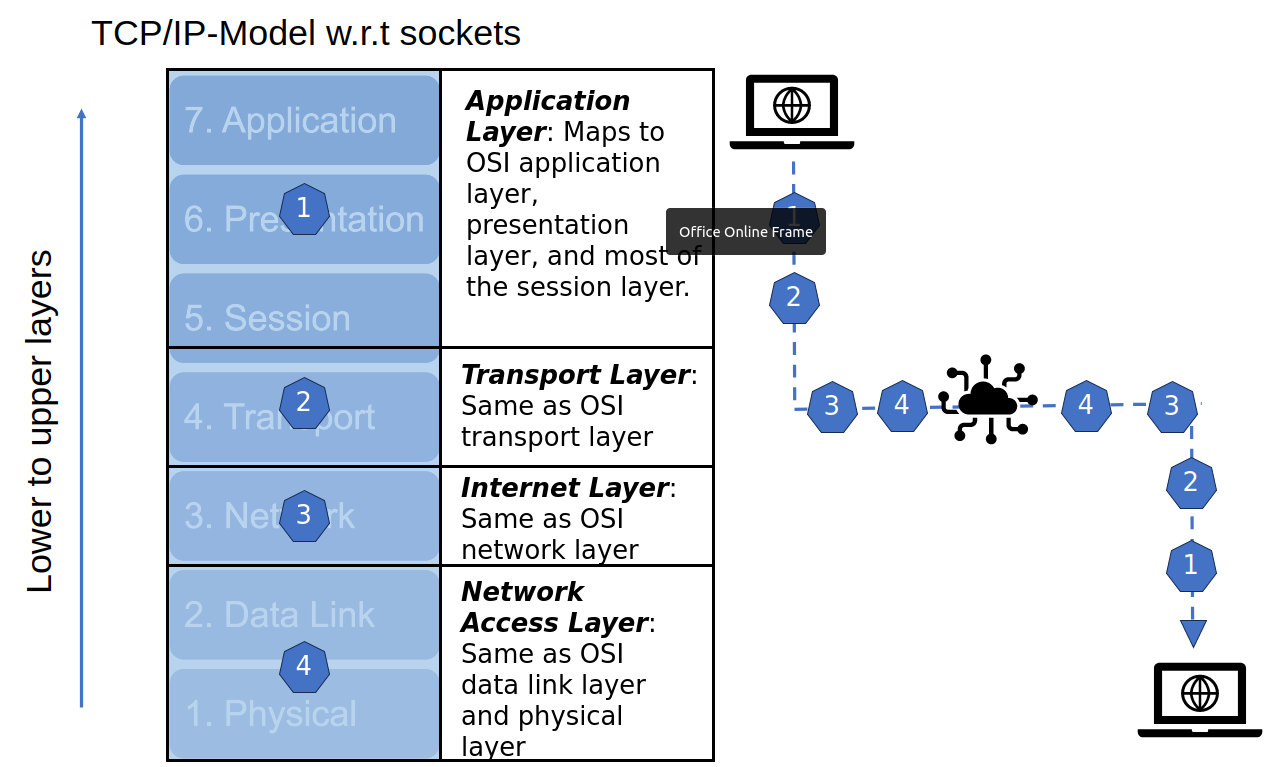
\includegraphics[width=\textwidth]{figures/TCP_IP.png}
    
    \centering
    \caption{\gls{tcp/ip} model with example protocols \label{fig: TCP_IP}}
\end{figure}

\subsection{Timing properties of data transfer w.r.t sockets and visual notations based on \gls{tcp/ip} model}
Since \gls{tcp} socket and WebSocket are operated in an application 
and the packet transfer of both will go through all layers in \gls{tcp/ip} model, 
a set of visual notations should be able to modularize the delays in each layer.
Thanks to the works of former researchers, there are already some graphical 
tools developed for difference purposes. The graphical tools 
can be roughly divided to two types, tools ideal for real world delay measurement 
for example the famous Wireshark, OPNET and NS-3, 
and tools suitable for modeling and visualization such as OpenModelica, 
Matlab/Simulink and LabVIEW, etc.



Although being out of scope of this thesis, the measurement of delay within 
each layer of \gls{tcp/ip} model will be essential for the future investment.
For instance, as depicted in figure \ref{fig: DSLConceptual}, the delay in 
each layer is represented as a block, which can be later integrated in graphical tools.
In this case, delay in a specific network layer will become comparable between
different technologies based on either application or transport layer protocols,
for example, \gls{tcp} socket and WebSocket. Apart from the network delay of
communication between agents, as shown in the figure, there are also other 
delay that can be modularized in the context of robot control. The robot 
control systems introduce delay first in \gls{rci} by executing the commands, 
and then a minor delay within the I/O module before activating the actuator.
After each robot motion driven by the actuator, its current state will be sent 
back to the \gls{cpu} by first going through the sensor, I/O module and \gls{rci} 
again. 







\begin{figure}[htb]
    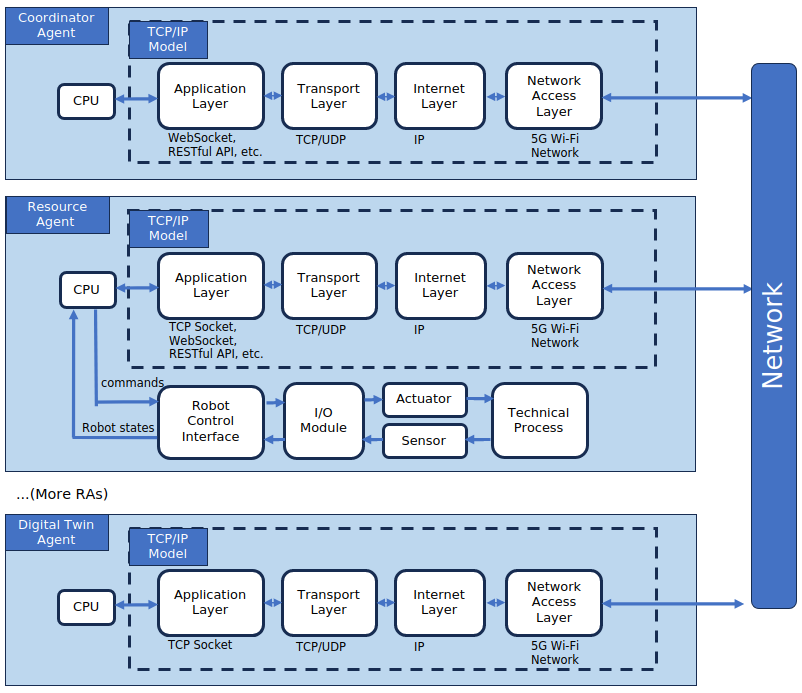
\includegraphics[width=\textwidth]{figures/DSLConceptual.png}
    
    \centering
    \caption{Conceptual diagram of a modularized general \gls{mas} based on \gls{dsl} \label{fig: DSLConceptual}}
\end{figure}
